% Chapter 1

\chapter{Introducción} % Main chapter title

\label{chap:Intro} % For referencing the chapter elsewhere, use \ref{Intr} 

%----------------------------------------------------------------------------------------

% Define some commands to keep the formatting separated from the content 
\newcommand{\keyword}[1]{\textbf{#1}}
\newcommand{\tabhead}[1]{\textbf{#1}}
\newcommand{\code}[1]{\texttt{#1}}
\newcommand{\file}[1]{\texttt{\bfseries#1}}
\newcommand{\option}[1]{\texttt{\itshape#1}}

%----------------------------------------------------------------------------------------

\section{Importancia del tema}
El conocimiento del medio ha sido tema de interés humano desde antaño. Lo que nos rodea, cómo se interactúa con ello en el día a día, así como poder investigar diferentes maneras en cómo se pueden aprovechar los recursos disponibles. \\

Los mapas realizados a mano, por ejemplo, en lugar de ser una herramienta de exactitud, son solo una referencia del entorno, dado el gran error derivado de la inexactitud humana en las mediciones. \\

Con el avance de la tecnología y el establecimiento de estándares, obtener herramientas de mejor presición ha sido cada vez más viable, y con ello, se puede obtener una mejor descripción del medio, acercándose a lo que en realidad es, y no a cómo lo interpreta la persona que realiza las mediciones. También, el desarrollo de computadores, sensores y actuadores ha permitido un menor sesgo en las mismas. 

\section{Planteamiento del Problema}
Los sistemas de medición actuales poseen cierto grado de incertidumbre, que en ocasiones resulta crítico dado el propósito para el que son utilizados, por ejemplo, en sistemas de tiempo real. \\

\begin{figure}[ht]
\centering
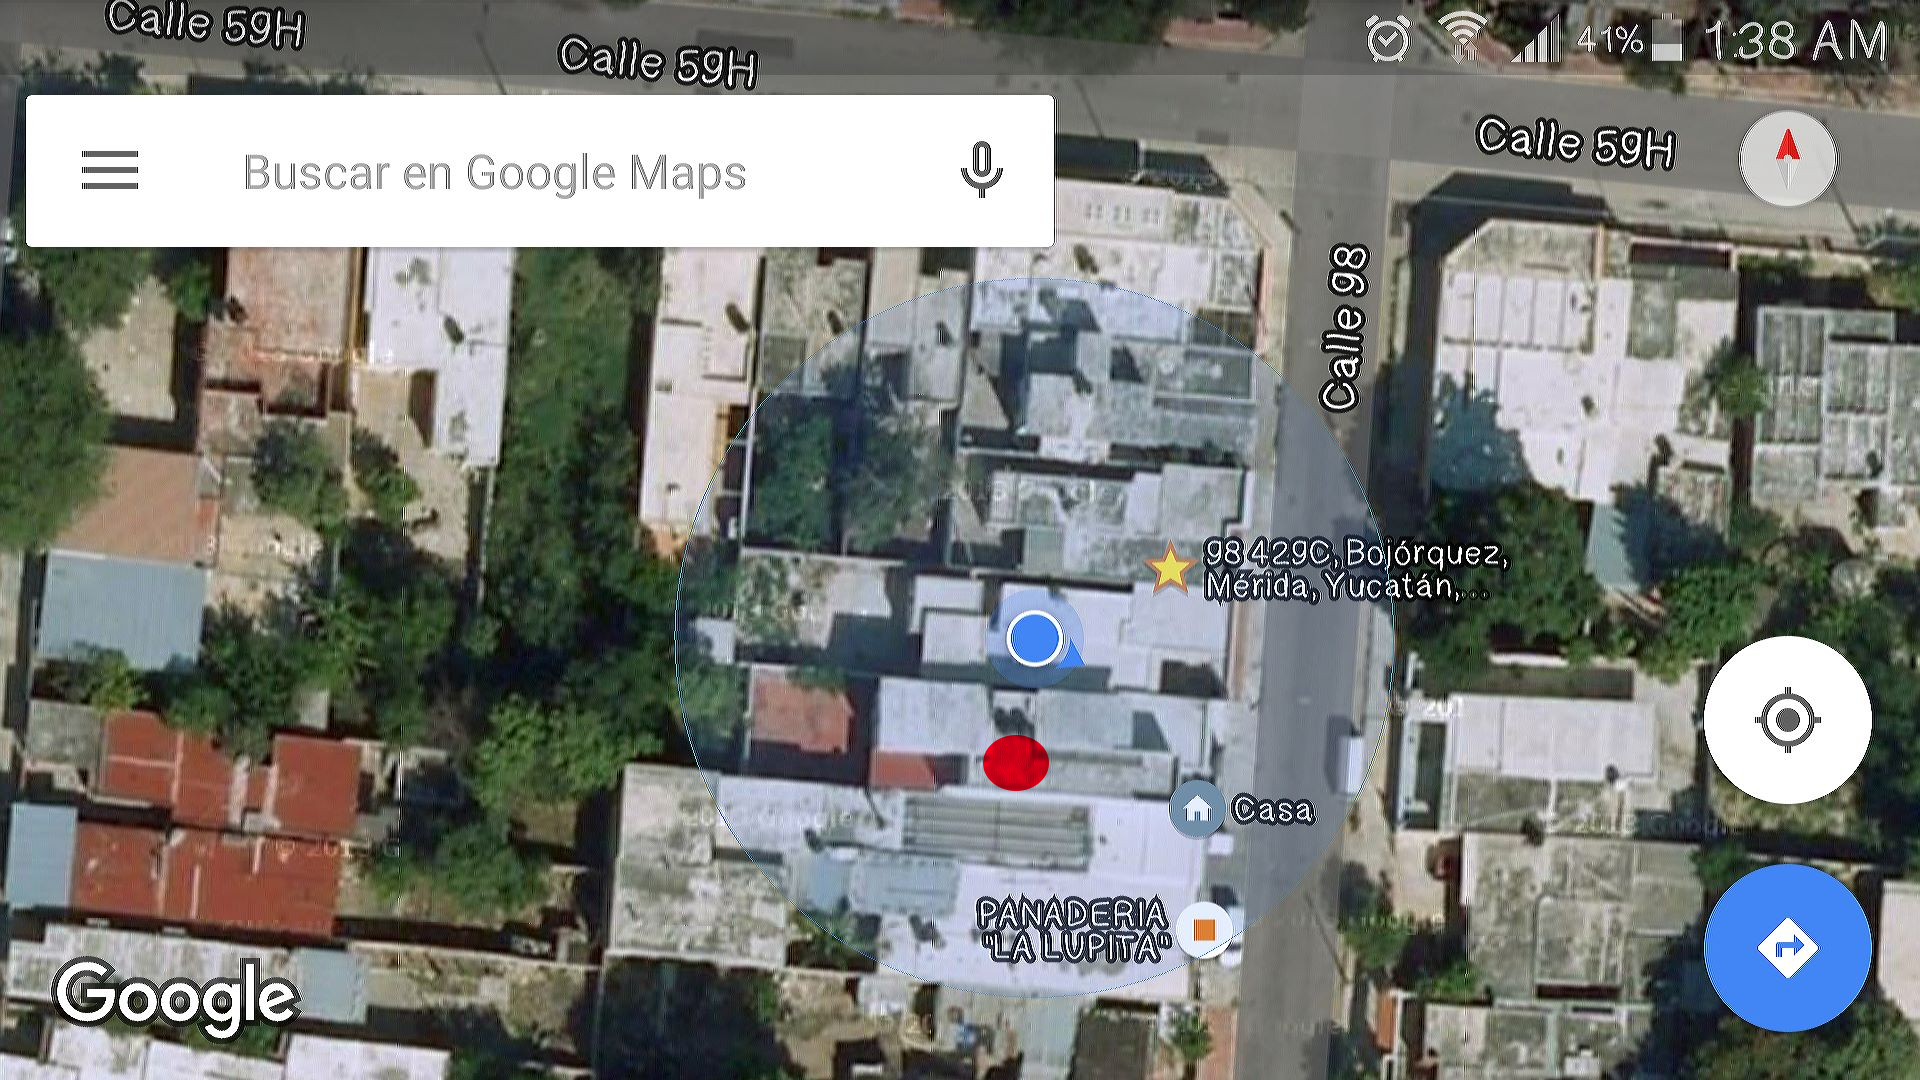
\includegraphics[scale=0.14]{Figures/Pred}
\caption[Posición de celular en mapa.]{Posición aproximada de la ubicación de un celular en un mapa de Google Maps.}
\label{fig:Prec}
\end{figure}

En una planeación de ruta de un sistema de navegación autónomo, una incertidumbre de $n$ metros a la redonda converge en una inexactitud significativa del sistema. El dispositivo puede encontrarse dentro de cualquier punto de la circunferencia de $2n$ metros de diámetro. Revise la figura~\ref{fig:Prec}, donde todo el círculo azul denota la posición aproximada de un dispositivo celular con GPS, y en donde la pequeña elipse roja muestra la posición real en dicho mapa. Además, cuando el sistema no está limitado a sólo seguir una ruta, sino que debe de ejecutar cierta acción cada determinados metros, entonces la incertidumbre se convierte en algo aún más crítico. Es evidente que el sistema no arrojará los resultados esperados debido a la falta de precisión.

\section{Trabajos previos}
En el trabajo \cite{de2011diseno}, se usa un sistema GPS (Global Positioning System, sistema de posicionamiento global, por sus siglas en inglés) para apoyar en la logística de distribución de farmacéuticos, como control de rutas, tiempos y seguridad, mencionando ante todo la capacidad de poder obtener los datos de localización y tiempo, además de la velocidad de desplazamiento de un vehículo. Sin embargo, de acuerdo al trabajo \cite{mendoza2004recomendaciones}, se propone una actualización del ancho de carriles carreteros a una amplitud adecuada máxima de 3.6 m, y dado que un GPS mide su incertidumbre en metros dependiendo del ruido, entonces se está ante un problema que requiere de modelos y cálculos matemáticos extra para reducir dicho error de medición, que podría incluso indicar que el vehículo se encuentra fuera de la cinta asfáltica o circulando en una vía contraria. \\

También, la tesis \cite{ronnback2000developement}, menciona la implementación de un sistema de navegación inercial INS/GPS para un UAV (Unmanned Aerial Vehicle, vehículo aéreo no tripulado, por sus siglas en inglés). Entre los datos a destacar, la posición de este sistema es estimada con un error de 2 metros con un 95\% de confianza, además de otros datos para asistir al vuelo como velocidad y su altitud. \\

Revisando el desarrollo \cite{maldonado2010controlador}, los autores afirman que las coordenadas recibidas de un dispositivo GPS solamente son usadas como aproximación a la posición del vehículo, y nunca como un dato sólido que sirviese al computar datos, dada la exactitud mínima de 10 metros. Sin embargo, mencionan limitantes tales como el peso total de la carga del UAV y el consumo de energía causado por la integración de todos los demás sensores, de donde el GPS aporta entonces una cantidad mínima de información y utilidad en general. \\


\subsection{Propuesta}
Dado que en los trabajos previos se presentan algunos inconvenientes con la presición del sistema de navegación inercial de los dispositivos dada la naturaleza del sensor GPS común utilizado, o bien, se requiere una fuerte cantidad de cálculos matemáticos en filtros para aún así seguir recibiendo errores medibles en metros, se propone la realización de un sistema de navegación que utilice una aplicación de cómputo denominada RTKLIB, que nominalmente reduce el error a una escala medible en centímetros a partir de dos señales de GPS, en un sistema portátil de arquitectura ARM, ampliando las posibilidades de aprovechamiento de los datos.

\section{Objetivo}
\subsection{General}
El objetivo general de este trabajo es el diseño y la implementación de un sistema de navegación capaz de conocer su ubicación en un entorno geográfico con una alta precisión para apoyar en proyectos que requieran de dicha información, utilizando un equipo pequeño y portátil.

\subsection{Objetivos específicos}
\begin{itemize}
    \item Configurar la transferencia de datos en UHF (Ultra-High Frequency, ultra alta frecuencia por sus siglas en inglés).
    \item Configuración de los equipos GPS.
    \item Acondicionamiento de una microcomputadora BeagleBone con sus respectivos periféricos de apoyo.
    \item Unificación de todos los módulos.
	\item Evaluación de los datos obtenidos.    
\end{itemize}
